\chapter{Stato dell'arte}
Illustriamo ora lo stato dell'arte relativo alle Cycle Generative Adversarial Networks (GAN), delle reti di Deep Learning in grado di tradurre immagini da un insieme ad un altro. Verranno analizzate le architetture sulle quali si basano queste reti e i concetti teorici che le caratterizzano. Inoltre verrà trattato un algoritmo per la rappresentazione visiva di come agiscono queste reti: GradCam.

\section{Machine Learning}
\emph{
    \textquotedblleft Si dice che un programma apprende dall'esperienza E con riferimento a alcune classi di compiti T e con misurazione della performance P, se le sue performance nel compito T, come misurato da P, migliorano con l'esperienza E.\textquotedblright
}
    \begin{flushright}
        \emph{Tom Mitchell \cite{tom1997hill}}
    \end{flushright}
Il Machine Learning è una branca dell'intelligenza artificiale che basa il suo funzionamento sulla capacità di apprendere dai dati e dalle esperienze passate \cite{mohri2018foundations}.
Sostanzialmente il Machine Learning cerca di insegnare ai computer a comportarsi come gli esseri umani: imparando dall'esperienza. Esso infatti non è altro che un metodo di analisi dei dati automatizzato che preso un set di dati in ingresso è in grado di effettuare una previsione su di esso basandosi su un modello.
Per capire meglio il concetto aiutiamoci con un esempio: supponiamo di dover creare un sistema in grado di rilevare la presenza di un cavallo all'interno di un'immagine. Questo compito, svolto da un essere umano dotato di pensiero, è un compito molto semplice: il nostro cervello sa com'è fatta la fisionomia di un cavallo, non deve far altro che confrontare l'immagine che vede con ciò che ricorda ed infine stabilire se è conforme o meno. Ora, supponiamo di voler sostituire l'essere umano con un computer, come facciamo a programmare una macchina per distringuere una foto con un cavallo rispetto a qualsiasi altra foto? L'idea è, appunto, quella di utilizzare un algoritmo di Machine Learning per addestrare il computer a rilevare l'animale. Rimanendo sull'analogia tra essere umano e computer, possiamo sfruttare il ragionamento di base dell'uomo e riportarlo sulla macchina: possiamo mostrare al computer tante immagini di cavalli come esempi, per far si che impari a riconoscerli. Per insegnargli a riconoscerle dovremo definire un insieme di parametri, detti features, utili al riconoscimento del cavallo. Possiamo, ad esempio, dire al computer di verificare la fisionomia delle orecchie, il colore del manto e la presenza o meno della criniera. Dovremo quindi verificare la presenza di tutti questi tratti e, infine, potremo determinare, con un margine di errore, se la foto in questione ritrae o meno un cavallo.

\subsection{Addestramento e discesa del gradiente}
Andando più nel dettaglio, possiamo dire che, dato un insieme in ingresso $X$ composto dagli esempi e dalle features che il modello deve estrarre e un insieme in uscita $Y$, composto dai valori che l'uscita può assumere (1 se presente il cavallo oppure 0, nel nostro caso di esempio), stiamo cercando una funzione $f(x)$ tale per cui: $$f(x): X \rightarrow Y$$
ovvero un'applicazione che associ ai valori $x$ un'uscita $y$.
\\Per ricavare l'applicazione cercata dovremo associare dei pesi $w$ alle features, tali per cui: $$y = w\textsubscript{1}x\textsubscript{1} + w\textsubscript{2}x\textsubscript{2} + ... +
w\textsubscript{n}x\textsubscript{n}$$ 
Dobbiamo quindi trovare il valore ottimo dei pesi in questione e lo facciamo attraverso l'addestramento della rete: partendo con pesi dal valore casuale, per ogni esempio, calcoliamo l'uscita $y$ e la confrontiamo con il valore associato all'esempio, al fine di calcolare la funzione d'errore (che ci indica, per l'appunto, quanto siamo distanti dal valore corretto). Una volta ottenuta la funzione d'errore possiamo calcolarne il gradiente rispetto ai pesi $w$, che ci indicherà la crescenza/descrescenza della funzione d'errore. Ora, sappiamo quanto vale la funzione d'errore, sappiamo qual è il suo gradiente, possiamo cercare di minimizzarla. Ci scosteremo quindi di un valore pari al \emph{learning rate}, un ulteriore parametro della rete, sulla funzione d'errore, e ripeteremo quanto fatto fino a quando non verrà trovato il valore minimo, che corrisponderà al valore ottimo dei pesi, come vediamo in figura \ref{fig:Discesa del gradiente}. Questo approccio viene denominato discesa del gradiente ed è utilizzato per addestrare le reti.
\begin{figure}[H]
  \begin{center}
    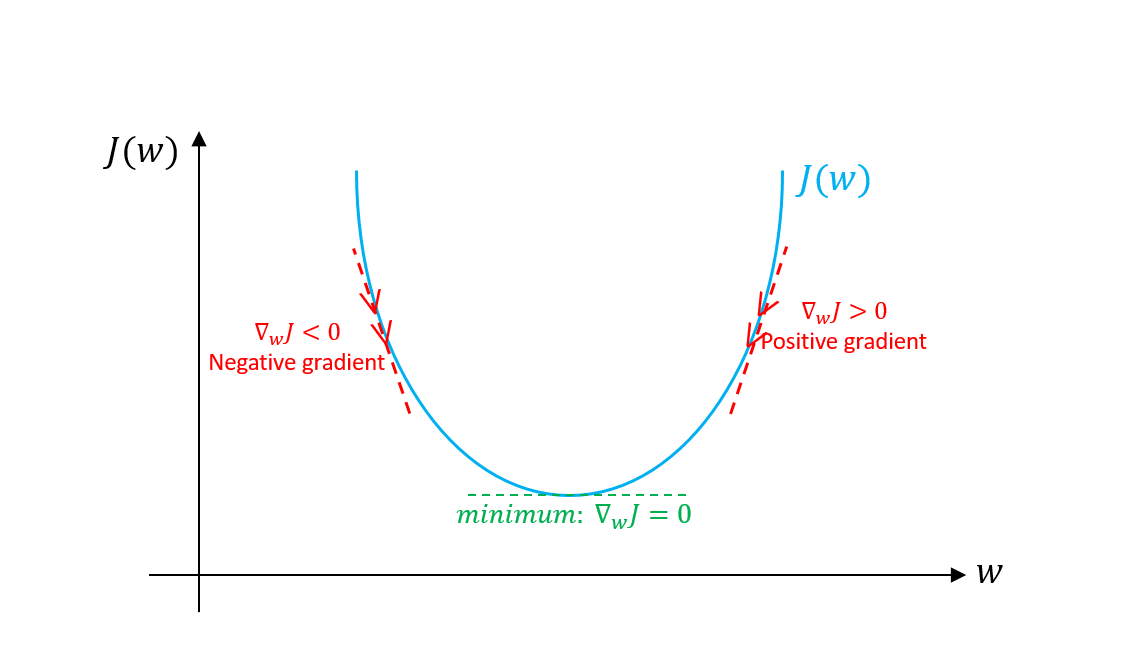
\includegraphics[width=0.8\columnwidth]{images/gradiente.png}
  \end{center}
  \caption{Vediamo come data una funzione, attraverso questo approccio si possa trovare il valore minimo.}
  \label{fig:Discesa del gradiente}
\end{figure}


\section{Deep Learning e Reti Neurali Artificiali}
Il Deep Learning è una branca del Machine Learning che mira ad estrarre delle rappresentazioni dei dati partendo dai dati stessi \cite{lecun2015deep}. La differenza sostanziale rispetto al Machine Lerning sta nel modo in cui vengono estratte le features: se nel Machine Learning occorreva la descrizione di un modello su cui basarsi per estrarle, con il Deep Learning non sarà più necessario. Le reti di Deep Learning infatti sono in grado di estrarre in modo del tutto autonomo queste features. Ovviamente per fare ciò occorre un enorme quantitativo di dati in più rispetto al Machine Learning ed è questo il motivo per il quale il Deep Learning si è sviluppato solo nell'ultimo periodo.

\begin{figure}[H]
  \begin{center}
    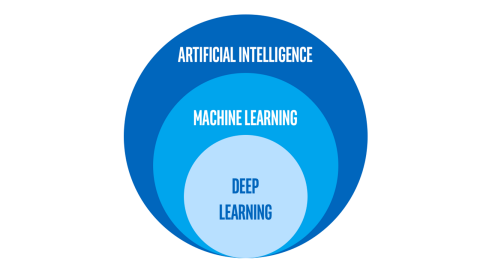
\includegraphics[width=0.8\columnwidth]{images/ai-machine-learning-deep-learning-rwd.png.rendition.intel.web.480.270.png}
  \end{center}
  \caption{Dalla figura capiamo come intelligenza artificiale, Machine Learning e Deep Learning siano strettamente connessi.}
  \label{fig:Artificial Intelligence Diagram}
\end{figure}

Le reti di Deep Learning sono costituite da strati detti \emph{layer}. In un algoritmo di Deep Learning ogni layer ha il compito di estrapolare una caratteristica specifica. Nelle elaborazioni delle immagini, ad esempio, i layer più bassi andranno a definire i bordi e le sfumature dell'immagine, mentre i layer più alti andranno invece a rilevare i concetti rilevanti per l'uomo, come la presenza di un viso o di una lettera.
Infine, per concludere questa panoramica iniziale sul Deep Learning occorre specificare cosa si intenda per \emph{hidden layer}, ovvero i layer nascosti. Gli hidden layer sono i layer interni alla nostra rete neurale, sono quei layer che mettono in comunicazione il primo layer, detto layer di input, con l'ultimo layer, detto layer di output, responsabile della produzione del risultato. Generalmente, per una rete neurale \emph{tradizionale} i layer nascosti sono 2-3, mentre per una rete neurale \emph{profonda}, tipica del Deep Learning, si arriva addirittura a 150 layer nascosti.
\\Vediamo ora come sono composti questi layer. Dicevamo come il compito di riconoscere un animale in foto fosse molto semplice da un punto di vista umano, mentre molto complesso per una macchina. L'ideale sarebbe avere una macchina dotata di \emph{cervello}, o comunque in grado di emulare il pensiero umano. E' proprio questa l'idea che è alla base delle reti neurali artificiali, ovvero le reti che vanno a comporre gli algoritmi di Deep Learning.
Le reti neurali umane sono un insieme di neuroni tra loro connessi, in grado di scambiare informazioni e di attivarsi o meno a seconda delle situazioni \cite{mehrotra1997elements}. Ricorda qualcosa? Esatto, è la funzione che hanno i layer in una rete di Deep Learning. Una rete neurale artificiale, è, quindi, un'emulazione delle reti neurali umane, composta da un grafo connesso di nodi, come si nota dalla figura \ref{fig:Artificial Neural Network}, all'interno del quale viaggiano le informazioni, o meglio i dati.

\begin{figure}[H]
  \begin{center}
    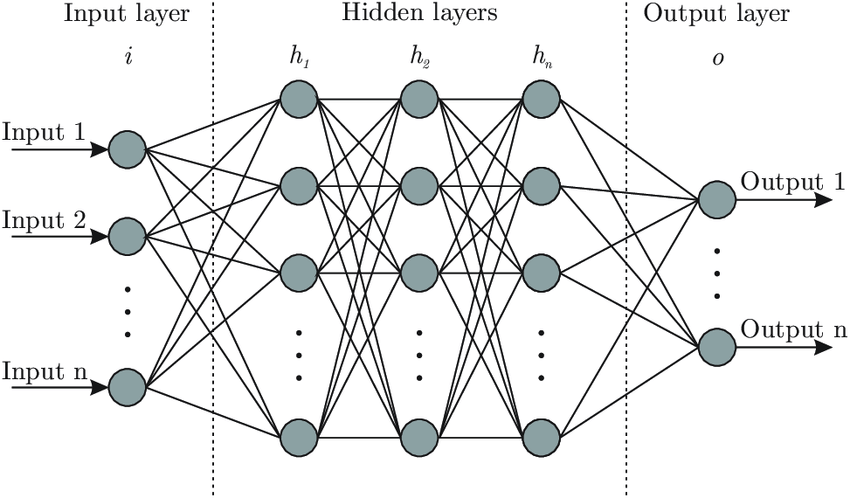
\includegraphics[width=0.8\columnwidth]{images/Artificial-neural-network-architecture-ANN-i-h-1-h-2-h-n-o.png}
  \end{center}
  \caption{Un esempio di rete neurale artificiale, notiamo la suddivisione in layer e come ogni neurone sia connesso ai neuroni del layer successivi}
  \label{fig:Artificial Neural Network}
\end{figure}

\section{Reti Neurali Convolutive}
Tra i tipi di reti neurali le rete neurali convolutive (CNN) sono le reti su cui fare riferimento quando si parla di visione artificiale ed elaborazione delle immagini \cite{yamashita2018convolutional}. Sono infatti reti in grado di catturare con successo ed efficienza le dipendenze spaziali e temporali delle immagini. Sono composte da tre blocchi o livelli: blocco convolutivo, blocco di pooling e i livelli completamente connessi. I primi due blocchi hanno il compito di estrarre le features, mentre il terzo ha il compito di mappare le features estratte nell'output finale. 
\\Per capire il loro funzionamento occorre analizzare come è definita un'immagine. Un'immagine non è altro come un insieme di pixel, ognuno con un determinato valore. Possiamo quindi vedere le immagini come una  matrice composta dai valori che assumono i pixel. Le immagini non sono però bidimensionali, infatti le immagini a colori sfruttano i tre canali RGB per comporre i colori, in questo caso avremo quindi una matrice con una dimensione tre di profondità, una per ogni canale. Per intenderci, un'immagine 4K avrà una definizione pari a 4096×2048, un numero quindi elevatissimo di pixel. E' proprio sulla dimensione che andremo a lavorare con il primo blocco delle rete neurali convolutive: vengono ridotte le dimensioni della matrice attraverso un'operazione di convoluzione, che dà il nome al blocco. Per descrivere il funzionamento definiamo il componente che ci permetterà di lavorare sulla matrice: il kernel, chiamato anche filtro. Il kernel può essere descritto come una matrice di pesi tipicamente di dimensione 3x3:
$$\begin{bmatrix}
w\textsubscript{11} & w\textsubscript{12} & w\textsubscript{13}\\
w\textsubscript{21} & w\textsubscript{22} & w\textsubscript{23}\\
w\textsubscript{31} & w\textsubscript{32} & w\textsubscript{33}
\end{bmatrix}$$
\\Il kernel ci permetterà di scorrere tutta l'immagine in altezza ed in larghezza, spostandoci ogni volta di una lunghezza definita a priori, e moltiplicare i valori con i pesi corrispondenti. Successivamente, questi valori verranno tra loro sommati ed andranno a comporre il nuovo valore della nuova matrice risultato, che avrà l'aspetto della figura \ref{fig:Kernel}.

\begin{figure}[H]
  \begin{center}
    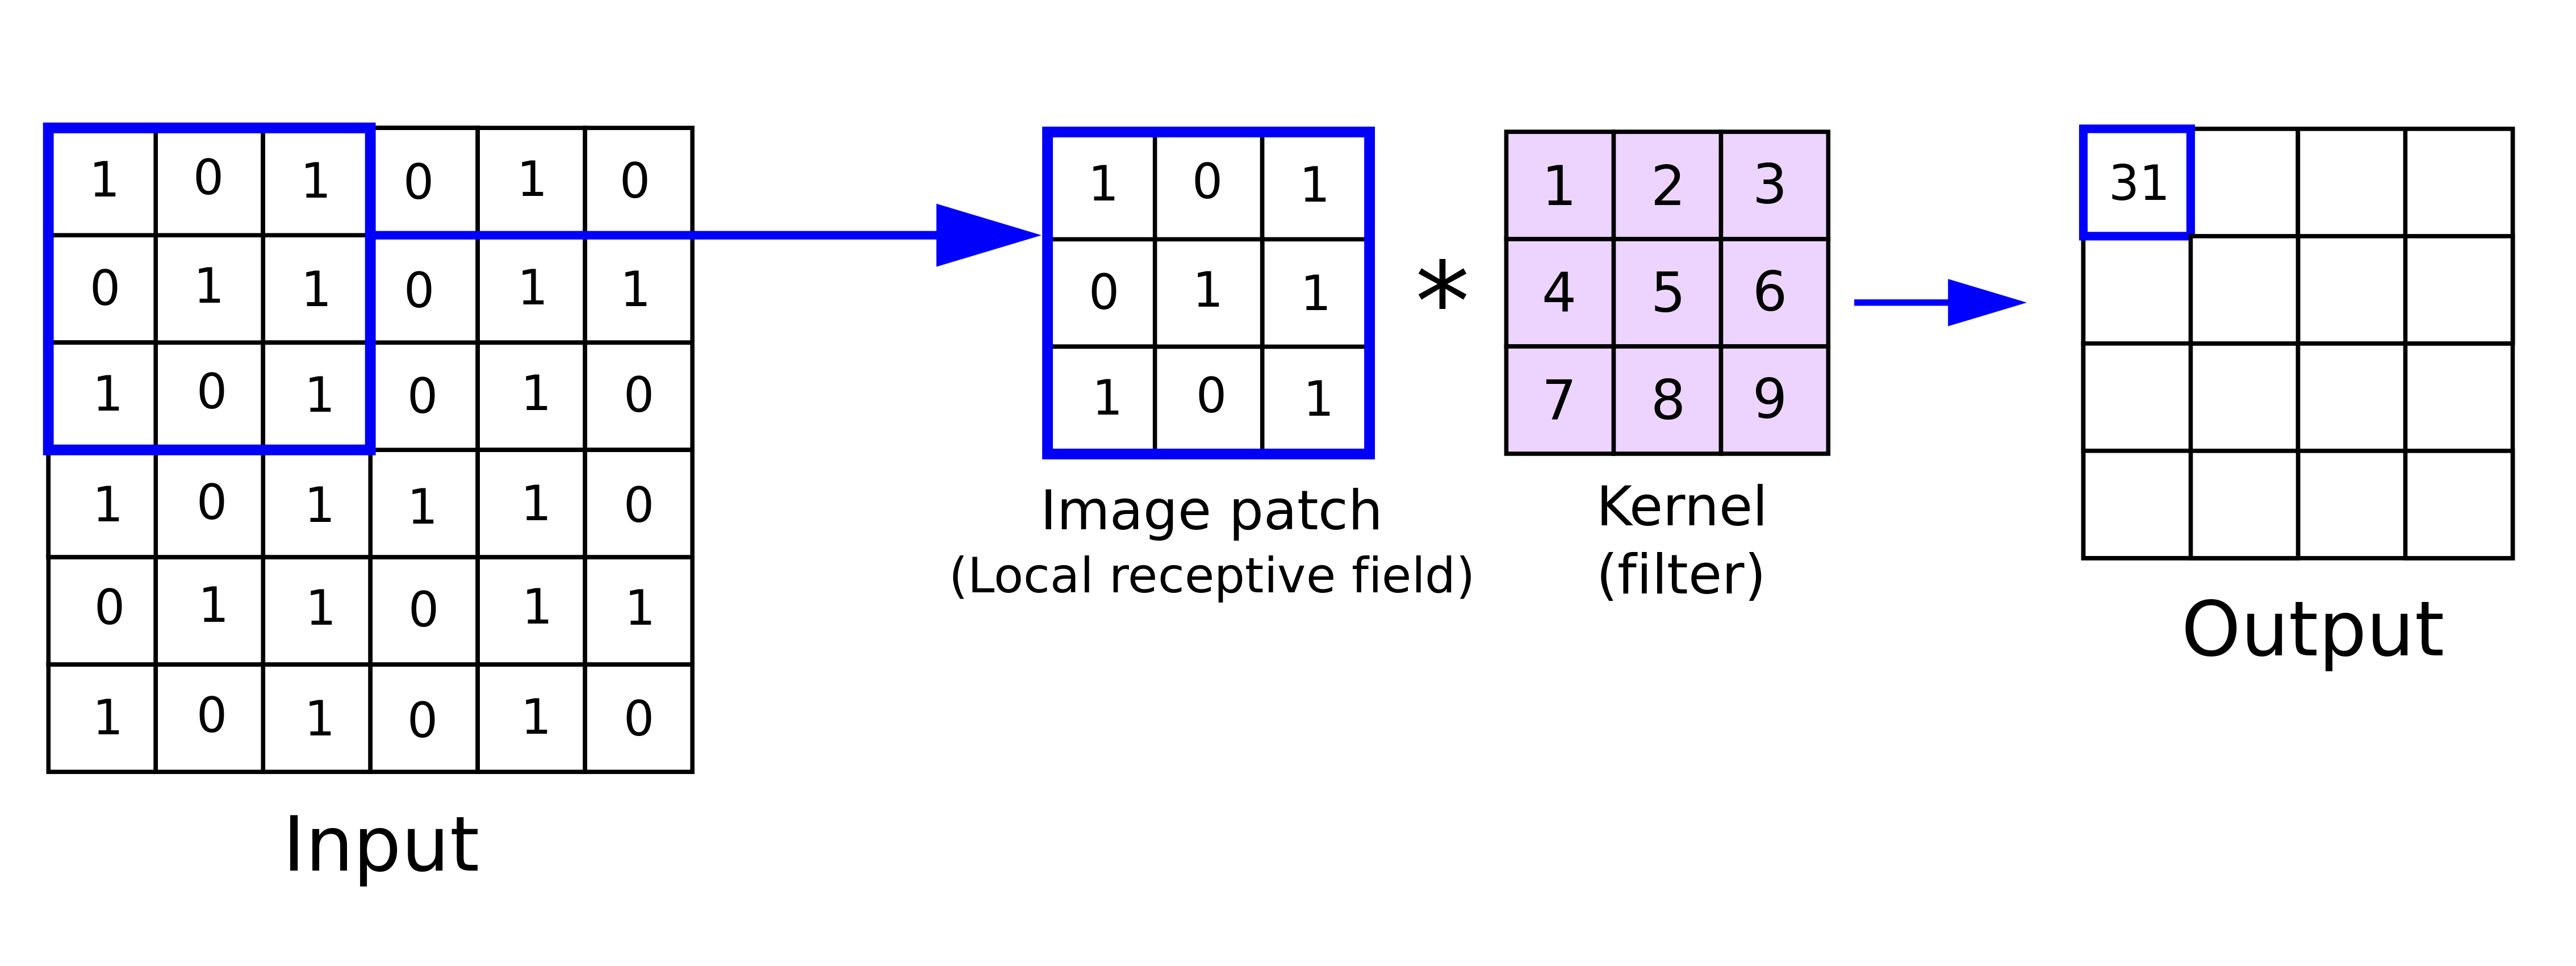
\includegraphics[width=0.8\columnwidth]{images/kernel.png}
  \end{center}
  \caption{Il kernel scorrerà tutta l'immagine al fine di creare una nuova matrice formata dalla somma dei valori dei pixel moltiplicati per i pesi.}
  \label{fig:Kernel}
\end{figure}
Quello che sta realmente accadendo è un'operazione di convoluzione sull'immagine al fine di rilevare caratteristiche come bordi, colore ed orientamento del gradiente.
Vi sono due tipi di approcci per questa operazione: il primo approccio, detto \emph{valid padding} permette di ottenere un risultato avente dimensione diversa rispetto alla matrice di partenza, mentre il secondo \emph{same padding} permette, aggiungendo ai margini della matrice iniziale colonne e righe composte da zeri, di ottenere una matrice avente la stessa dimensione di quella di partenza. Durante l'addestramento della rete, lo scopo sarà quello di trovare i valori dei pesi per i quali il kernel fornisce i risultati migliori. Dopo un'operazione di questo tipo, l'output viene fatto passare attraverso una funzione di attivazione, tipicamente una \emph{ReLu} che eliminerà i valori negativi.
\\Il secondo blocco, di pooling, avrà il compito di ridurre le dimensioni ulteriormente, al fine di ridurre la potenza di calcolo necessaria ad elaborare i dati, estrarrà le caratteristiche dominanti ed effettuerà una riduzione del rumore. Il compito di questo blocco sarà quello di ridurre le dimensioni della matrice e raggruppare i valori grazie all'utilizzo di un filtro unitario. Il filtro scorrerà tutta la matrice e, per ogni scorrimento, calcolerà un valore, che sarà il valore che andrà a comporre il risultato. Questo valore può essere calcolato secondo due approcci: \emph{max pooling} dove per ogni raggruppamento il risultato sarà il valore massimo, come in figura \ref{fig:Pooling}, oppure \emph{average pooling} dove per ogni raggruppamento il risultato sarà la media dei valori.
\begin{figure}[H]
  \begin{center}
    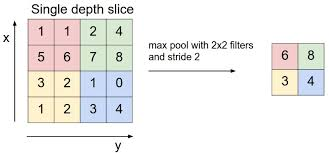
\includegraphics[width=0.8\columnwidth]{images/pooling.jpg}
  \end{center}
  \caption{In questo caso viene applicato l'approccio max pooling, vediamo come il filtro di dimensione 2x2 ricavi nel primo quadrante della matrice il valore massimo 6 e lo vada ad inserire nella matrice risultato.}
  \label{fig:Pooling}
\end{figure}
Abbiamo visto quindi come vengano catturate le caratteristiche principali della nostra immagine grazie ai primi due blocchi della rete, ora il compito passerà all'ultimo blocco il quale avrà il compito di convertire i risultati fin'ora ottenuti nella forma adatta agli output finali della rete.
\\Le CNN sono molteplici, successivamente ci concentreremo sull'architettura ResNet che descrive la rete del nostro progetto.


\section{Generative Adversarial Network}
Le Generative Adversarial Netwrok (GAN) sono un modello generativo basato sul Deep Learning \cite{brownlee2019generative} utilizzato per la creazione di immagini. Si tratta di un modello basato su due reti: una rete discriminativa, che ha lo scopo di determinare se un'immagine è reale, oppure falsa, ed una rete generativa, il quale compito è appunto quello di generare immagini. Per capire meglio il loro funzionamento aiutiamoci con un paragone: la rete discriminatrice possiamo vederla come un poliziotto, mentre la rete generatrice come un contraffattore. Lo scopo del contraffattore è quello di affinare la propria abilità al fine di produrre opere false e riuscire a spacciarle per vere senza farsi scoprire, mentre lo scopo del poliziotto è quello di ostacolare il contraffattore rilevando se un'opera è reale o meno. La competizione generata da questo duello porta entrambi a migliorarsi, fino a quando non si arriverà al punto in cui il contraffattore riesce a riprodurre opere indistinguibili da quelle reali \cite{goodfellow2014generative}.
\\
Andiamo ora a descrivere queste reti e la teoria sulla quale si basano.
\\Prima di tutto occorre parlare di una tipologia differente da quella fin'ora trattata di addestramento: l'addestramento non supervisionato. Abbiamo visto come durante la fase di addestramento gli esempi forniti alla rete vengano associati ad un valore di uscita $y$ e di come la rete si addestri su questi valori. Nell'addestramento non supervisionato, a differenza, agli esempi di addestramento, non vengono associate le uscite $y$, ma vengono forniti solo gli input. L'obiettivo di questo addestramento è quello di rendere la rete in grado di rilevare una correlazione tra gli esempi e, di conseguenza, di ricavare un modello. E' ciò che sta alla base dei modelli generativi, ovvero i modelli in grado di generare nuovi elementi il quanto più possibile simili agli elementi dell'insieme di input.
\\
Dicevamo di come il modello fosse suddiviso in Generatore e Discriminatore, andiamo ora a vedere come lavorano.
\\Partendo inizialmente da un vettore casuale $z$, il generatore $G$ genererà un'immagine fake $G(z)$. Questa immagine sarà poi data in ingresso al Discriminatore $D$, che dovrà determinare se l'immagine è reale o falsa, dovrà quindi fare una predizione $D(G(z))$. Sul risultato di questa previsione verrà calcolata la funzione d'errore del discriminatore e, con il metodo già ampiamente descritto della discesa del gradiente, verrà addestrato, mantentenendo invariati i parametri del Generatore. Sempre con lo stesso metodo verrà successivamente addestrato il Generatore.
\\Le funzioni d'errore utilizzate nell'addestramento di queste reti sono logaritmiche. Supponiamo il caso di un'immagine reale, i casi possono essere due:
\begin{itemize}
    \item la previsione è conforme all'immagine, ovvero, determinato con 1 il valore dell'immagine reale, la previsione sarà un valore ad esso vicino, ad esempio $D(x)=0.9$, per cui l'errore commesso sarà piccolo
    \item la previsione è errata, ad esempio $D(x)=0.1$, per cui l'errore commesso sarà grande
\end{itemize}
Una funzione che si comporta come quanto descritto è $f=-log(D(x))$, che nel nostro caso avrà come risultato: $f=0.1$ per $D(x)=0.9$ e $f=2.3$ per $D(x)=0.1$. Come visto questa funzione approssima bene il comportamento che vogliamo ottenere dalla funzione d'errore, ovverò è elevata tanto più la previsione è errata.
\\Con calcoli analoghi, si ottiene come risultato $f=-log(1-D(G(z))$ nel caso in cui l'immagine sia generata dal Generatore. Quindi, dato che l'obiettivo della rete è quello di generare un'immagine finta indistinguibile da una reale, l'apprendimento consisterà quindi nell'ottimizzare un gioco \emph{minmax} per $G$ e $D$:
$$
{\displaystyle \min _{G}\max _{D}\mathbb {E} _{{\boldsymbol {x}}\sim p_{data}({\boldsymbol {x}})}[\log D({\boldsymbol {x}})]+\mathbb {E} _{{\boldsymbol {z}}\sim p_{\boldsymbol {z}}({\boldsymbol {z}})}[\log(1-D(G({\boldsymbol {z}})))]}
$$
\\L'utilizzo delle GAN si concentra su tre campi principali:
\begin{itemize}
    \item Image Super-Resolution, per migliorare la qualità delle immagini in ingresso;
    \item Creare arte;
    \item Image to Image Translation, ovvero l'applicazione di uno stile ad un'immagine di input, come ad esempio estate-inverno, giorno-notte, e, come vedremo più avanti nel nostro caso, cavallo-zebra. Un esempio di questa applicazione è mostrato in figura \ref{fig:HorsetoZebra Example}.
\end{itemize}

\begin{figure}[H]
  \begin{center}
    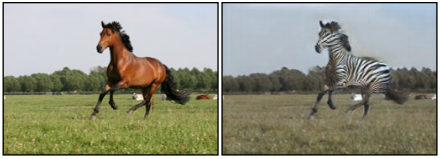
\includegraphics[width=0.8\columnwidth]{images/cyclegan example.png}
  \end{center}
  \caption{Un esempio di Image to Image translation  \cite{Zhu_2017_ICCV}}
  \label{fig:HorsetoZebra Example}
\end{figure}
\subsection{Pix2Pix Translation}
Un aspetto da sottolineare per quanto riguarda le GAN è la possibilità di condizionarne il funzionamento. Parliamo quindi di Conditional Generative Adversarial Network, utilizzate nella traduzione da immagine a immagine Pix2Pix \cite{goodfellow2014generative}.
\\Abbiamo visto come le GAN generino delle immagini partendo dal rumore. L'idea che è alla base di questa traduzione è quella di partire a generare un'immagine non più da un vettore casuale ottenuto dal rumore, bensì da un'altra immagine \cite{isola2018imagetoimage}. Aiutandoci con un esempio, supponiamo di avere una GAN utilizzata nella generazione di visi umani. Dalla GAN in questione ci aspettiamo che la probabilità di generare un volto femminile sia pari a quella di un volto maschile, e che quindi la rete non faccia distinzione sull'output generato. Utilizzando una GAN condizionata possiamo, appunto, condizionare la generazione dei volti solo su quelli femminili o solo su quelli maschili. Per fare ciò addestreremo la rete non più su una singola immagine come visto fin'ora, ma su coppie di immagini, grazie ad un dataset \emph{paired}, ovvero un dataset composto da immagini accoppiate a due a due secondo la relazione input-output \cite{Zhu_2017_ICCV}. In questo modo il discriminatore non lavorerà più facendo previsioni solamente sull'immagine generata, ma lo farà sulla coppia di immagini: immagine di partenza più immagine generata e immagine di partenza più rispettivo output, come si nota dall'esempio in figura \ref{fig:Pix2Pix}.


 \begin{figure}[H]
  \begin{center}
    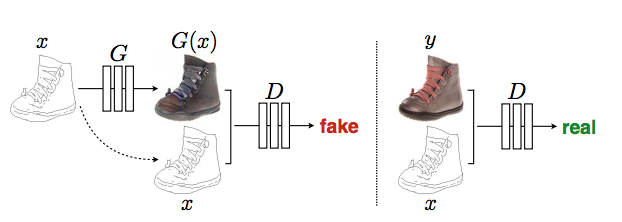
\includegraphics[width=0.8\columnwidth]{images/pix2pix.png}
  \end{center}
  \caption{Vediamo come il discriminatore esegua una previsione sulla coppia di immagini input-output fake e input-output associato.}
  \label{fig:Pix2Pix}
\end{figure}


\section{GradCam}
Abbiamo ampiamente parlato di CNN e di come il loro funzionamento sia ideale o molto performante nell'ambito della visione artificiale e dell'elaborazione delle immagini. Come per ogni ambito dell'intelligenza artificiale, è molto importante capire il loro funzionamento e renderle il più intuitive possibili. Questo perchè, nel caso di un malfunzionamento, occorre sapere da che cosa è stato determinato. La necessità di comprendere in maniera trasparente il loro funzionamento è data da tre principali motivi. In primo luogo, quando l'AI è debole rispetto alla capacità umana è utile identificare il perchè il suo comportamento fallisca. Successivamente quando l'AI è pari alla capacità umana l'obiettivo è quello di stabilire un'adeguata fiducia negli utenti. Infine, quando l'AI è decisamente superiore all'intelligenza umana l'obiettivo è quello di apprendere da essa \cite{Selvaraju_2017_ICCV}.
\\Una delle tecniche principali per capire il funzionamento delle CNN è attraverso le mappe di attivazione di classe (CAM). La loro logica è basata sui risultati che produce l'ultimo livello convolutivo di una CNN. Sostanzialmente, grazie alle features map prodotte dall'ultimo layer convolutivo è possibile ricavare dove si focalizza l'attenzione della rete. Per rendere più chiaro il concetto riprendiamo l'esempio della rete classificatrice. Vogliamo capire dove si concentra la rete, su che parametri dell'immagine. Ci aspettiamo che difficilmente l'attenzione sia focalizzata ai margini dell'immagine, o su parametri secondari come lo sfondo, ma che sia focalizzata sulla sagoma dell'animale. CAM ci permette, grazie ad una mappa del calore come vediamo in figura \ref{fig:GradCam example}, di verificare come si comporti la rete nell'analisi dell'immagine.

\begin{figure}[H]
  \begin{center}
    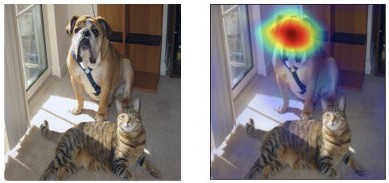
\includegraphics[width=0.8\columnwidth]{images/gradcam example.jpg}
  \end{center}
  \caption{Il risultato dell'applicazione di GradCam su una rete classificatrice. In questo caso l'output di classificazione riguarda il cane e vediamo come l'attenzione sia concentrata tutta sulla faccia dell'animale.}
  \label{fig:GradCam example}
\end{figure}
L'approccio visto fin'ora funziona però solo su reti CNN e non su altre architetture. Introduciamo quindi GradCam, avente un funzionamento simile a quanto descritto, ma applicabile a qualsiasi tipologia di architettura.
Vediamone il funzionamento nel dettaglio. Sia la nostra rete una rete classificatrice e sia $y\textsuperscript{c}$ l'output di classificazione della rete. Denotiamo inoltre con $A\textsuperscript{k}$ le mappe di attenzione generate dall'ultimo layer convolutivo della rete sulle quali vogliamo andare a calcolare l'attenzione. Calcoliamo il gradiente di $y\textsuperscript{c}$ rispetto alle mappe di attenzione $A\textsuperscript{k}$:
$$\frac{\partial y\textsuperscript{c}}{\partial A\textsuperscript{k}}
$$
Ora, applichiamo un \emph{global average pooling}, ovvero la media su altezza e larghezza di ogni mappa di attenzione, e poniamo:
$$\alpha\textsuperscript{c}\textsubscript{k} =
\frac{1}{Z} \sum_{i=1} \sum_{j=1} \frac{\partial y\textsuperscript{c}}{\partial A\textsuperscript{k}\textsubscript{ij}}$$
$\alpha\textsuperscript{c}\textsubscript{k}$ sarà un vettore di dimensione pari al numero di feature map del layer scelto e conterrà i pesi da affidare ad ogni feature map.
\\Successivamente moltiplicheremo il vettore contenente i pesi con le features map e ne faccremo una somma. In questo modo associamo ad ogni canale della convoluzione un peso determinato dal gradiente. Il peso associato a questi canali indica se si attivano o meno durante l'elaborazione dell'immagine. Infine applicheremo una ReLu alla somma ottenuta, al fine di eliminare i valori negativi. \\Il risultato ottenuto potrà essere visto attraverso una mappa del calore ed indicherà dove sarà maggiormente focalizzata l'attenzione della rete nel layer stabilito.

\section{Fréchet Inception Distance}
Definite le GAN, definito GradCam come metodo per visualizzare dove le reti vanno a lavorare, occorre ora definire un metodo per valutare la qualità della rete generatrice. Introduciamo quindi il Fréchet Inception Distance (FID). Il FID è un metodo utilizzano per valutare la qualità delle immagini generate da una GAN \cite{DBLP:journals/corr/HeuselRUNKH17}. Il metodo si basa sul concetto matematico della distanza di Fréchet utilizzato in matematica per calcolare la somiglianza tra le curve tenendo conto della posizione e dell'ordine dei punti lungo le curve \cite{eiter1994computing}. Il ragionamento è quello di valutare due insiemi: un insieme di esempio e un insieme di immagini generate dalla rete. Vengono calcolate quindi le distribuzioni di questi due insiemi, vengono confrontate e viene prodotto un risultato. Il risultato indicherà quanto sono distanti le due distribuzioni, quindi un risultato piccolo è ottimale. 